\subsection{Level2.2: $z=x^2 + y^2$ について}
\subsubsection{プログラムソース(変更部分)}
\begin{breakbox}
\begin{verbatim}
行数 変更点
32 z=x*x+y*y;
44  z_dx = 2*x*z_dx;
56 z_dy = 2*y*z_dy;
\end{verbatim}
\end{breakbox}

\subsubsection{観察意図と観察方法}

学習係数が探索挙動に及ぼす影響を確認するために,seed値とalpha値を変更し観察を行う.\\

\begin{enumerate}
\item alpha値を固定してseed値を変更する.\\
alpah値は0.1で固定,seed値は1~10,1000刻みの1000~10000とする.
\item seed値を固定してalpha値を変更する.\\
seed値は1で固定,alpha値は0.1~0.9とする.
\end{enumerate}

\subsubsection{実行結果}


1.seed値を変更したときのstep数.\\
step数に多少の変化がみられたものの,劇的な変化ではなかった.\\\\

2.alpha値を変更したときのstep数.\\
\begin{figure}[h]
 \begin{center}
  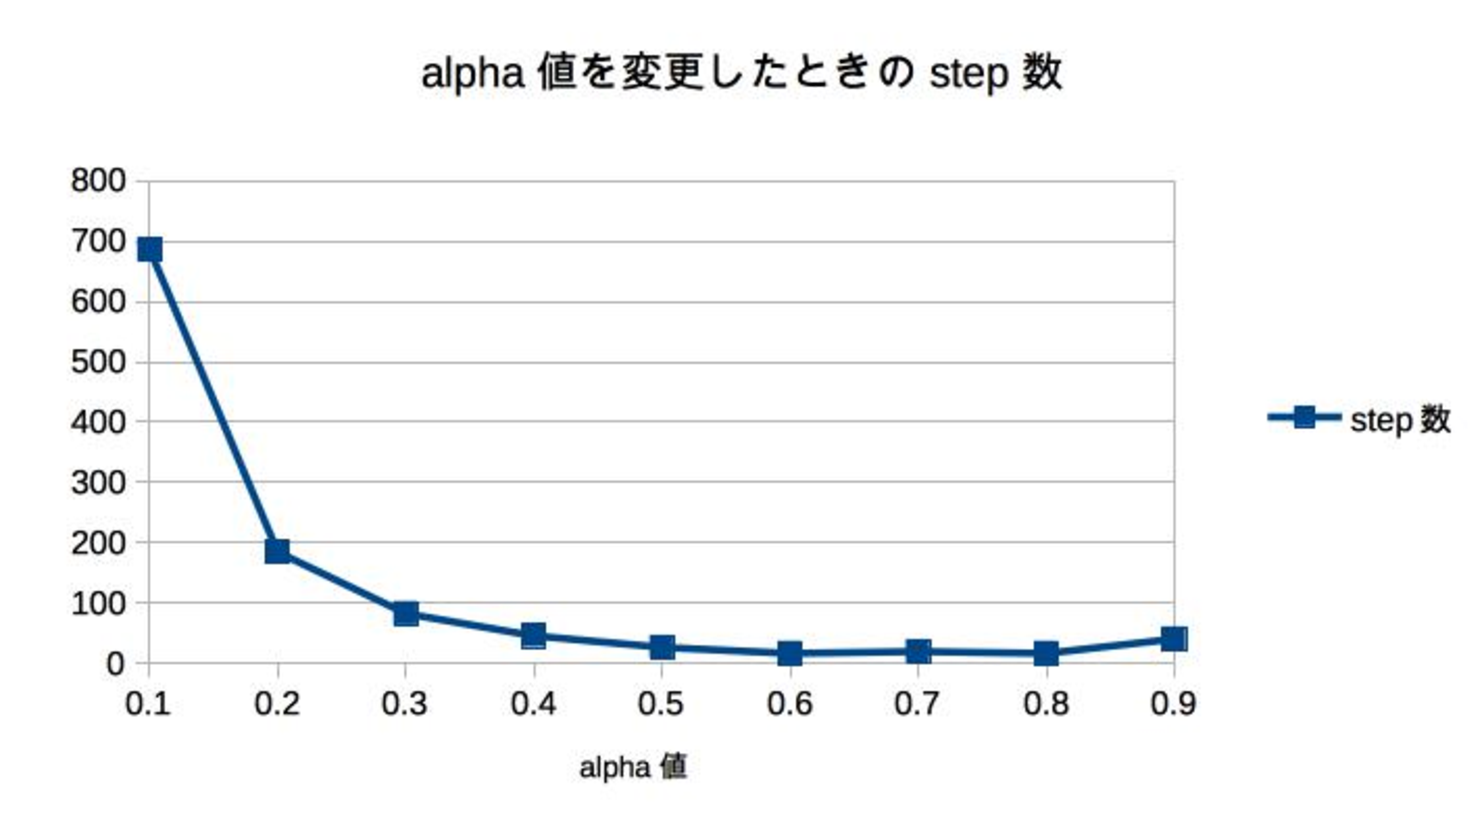
\includegraphics[width=10.0cm]{figs/level2.2/2.2alpha.pdf}
  \caption{step数の変化}
	\label{step_alpha}
 \end{center}
\end{figure}

alpha値を変更したことにより,step数に大きな変化がみられた.\\
特にalpha値を0.1から0.2に変化させたときにstep数の大幅な減少がみられる.\\\\

またstep数が変化すると探索ステップ数あたりの目的関数推移図にも変化が生じることがわかった.\\

\begin{figure}[h]
 \begin{center}
  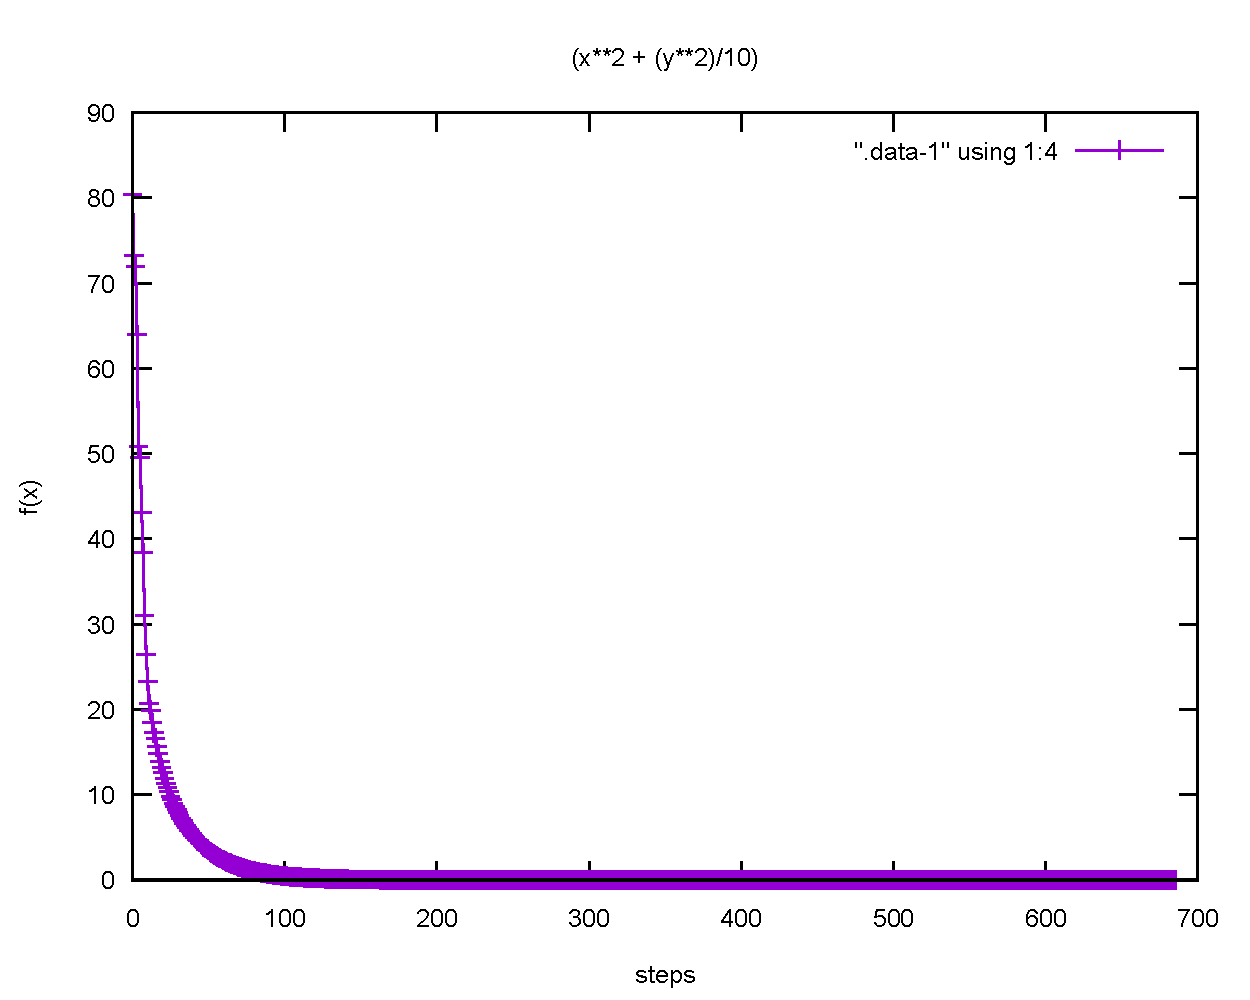
\includegraphics[width=10.0cm]{figs/level2.2/sim-1-2.pdf}
  \caption{alpha値0.1のときの推移図}
	\label{step_alpha}
 \end{center}
\end{figure}

\begin{figure}[h]
 \begin{center}
  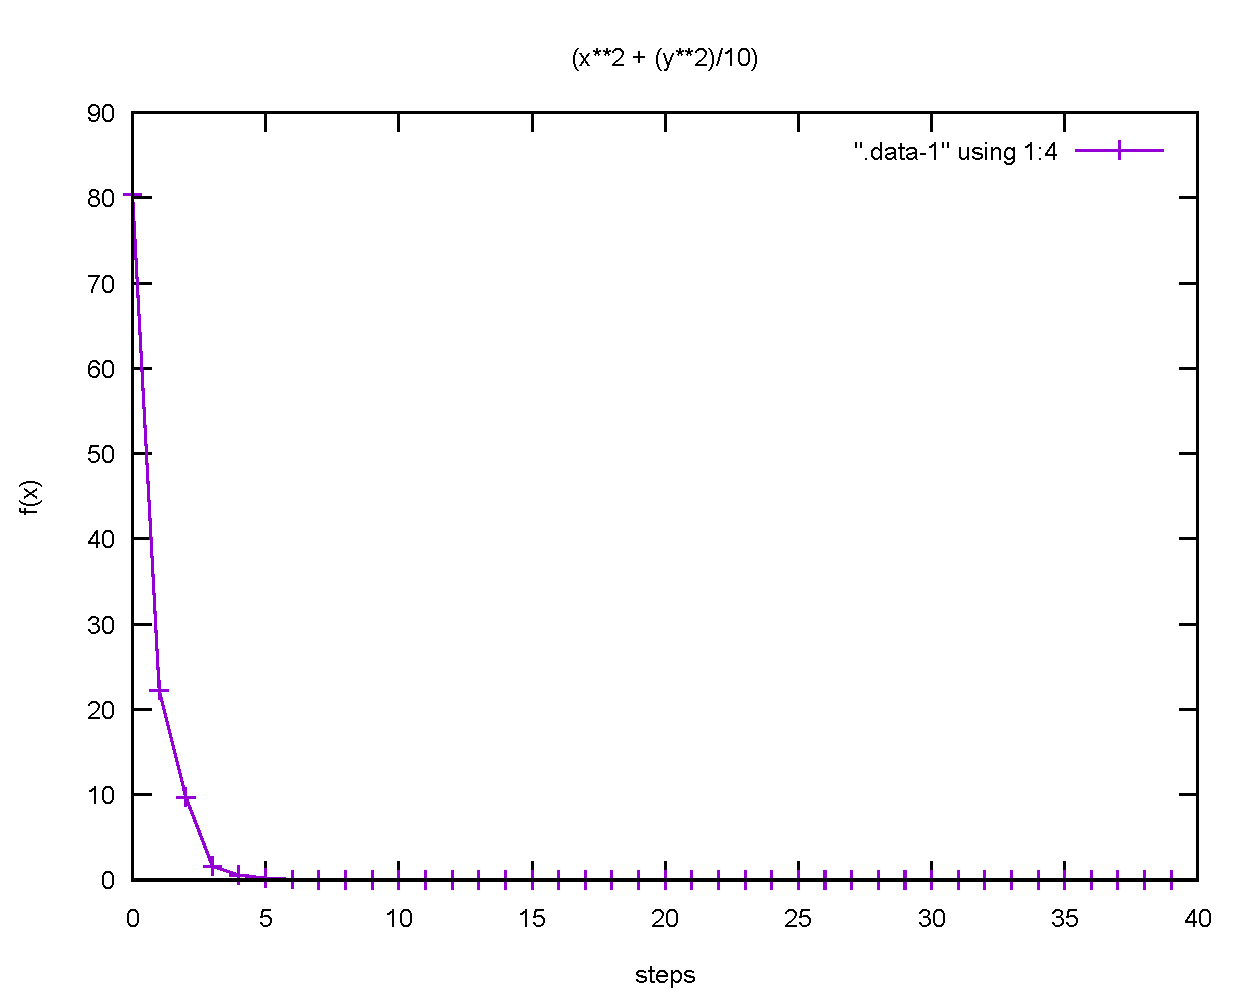
\includegraphics[width=10.0cm]{figs/level2.2/sim-1.pdf}
  \caption{alpha値0.9のときの推移図}
	\label{step_alpha}
 \end{center}
\end{figure}

alpha値0.1(step数が多い)ときのほうが図がなめらかである.

\subsubsection{考察}

学習係数を変化させることによりstep数を減らすことができた.探索回数が減ることにより効率はあがったと考える.\\
しかし,探索ステップ数あたりの目的関数推移図を見ると,step数が多いほうが探索点が最適解にたどりついたより正確な地点を知ることができると考える.



